\section{RTL Verification}
\label{sec:rtlverification}
The testbench for the register transfer level verification of count32 and memcpy46 sample test programs consists of the memory module and the cpu top module. The clock and reset signals are generated in the testbench module. The cpu module reads the instructions from the memory module, which is loaded with the initial date for the sample programs, and also saves the results of the program execustions in the memory.

In earlier stages of development, testbenches for the modules were used. After the modules were written and tested, they were integrated into the top module one by one and tested together. Before the integration of the instruction fetch module, the decoder and execution stage were tested together with different complicated instructions like IT, LDMIA and STMIA. The instructions were asserted directly in the testbench. The hex codes for the test programs were generated by the GNU ARM assembler which translated the written assembler test programs to the hex codes needed in the testbenches. C programs were unsuited for the testing at this stage because they did not necessarily generate the exact instruction sequences desired.

\begin{figure}
\centering
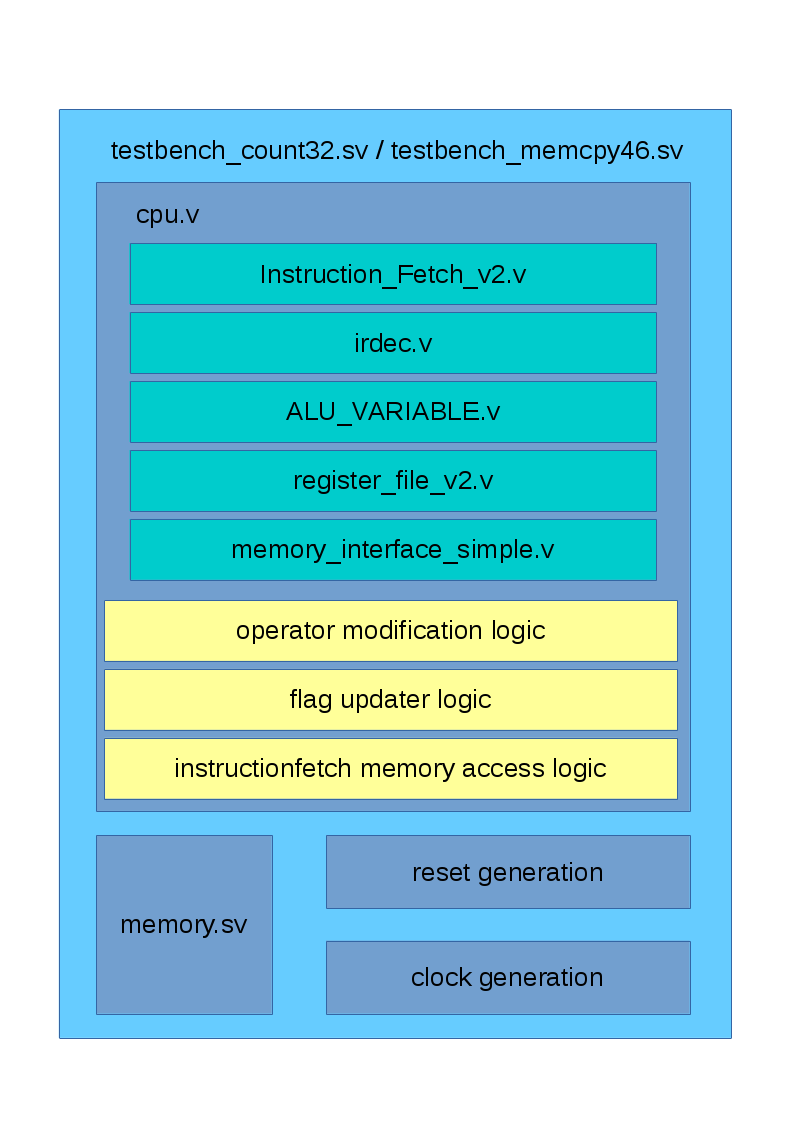
\includegraphics[scale=0.5]{images/rtltestbenchdrawing.png}
\label{fig:rtltestbenchdrawing}
\caption{Structure of the rtl top level testbench}
\end{figure}